\section{Convolutional Neural Networks for Dense Prediction}

\subsection{Encoder–Decoder Networks and U-Net}
A common way to adapt Convolutional Neural Networks (CNNs) for dense prediction is to use an \textbf{encoder–decoder structure}. The \textbf{encoder} progressively downsamples the input to build high-level, context-rich features, while the \textbf{decoder} upsamples these features back to the original resolution to produce a per-pixel output map \cite{31}. 

\begin{figure}[H]
    \centering
    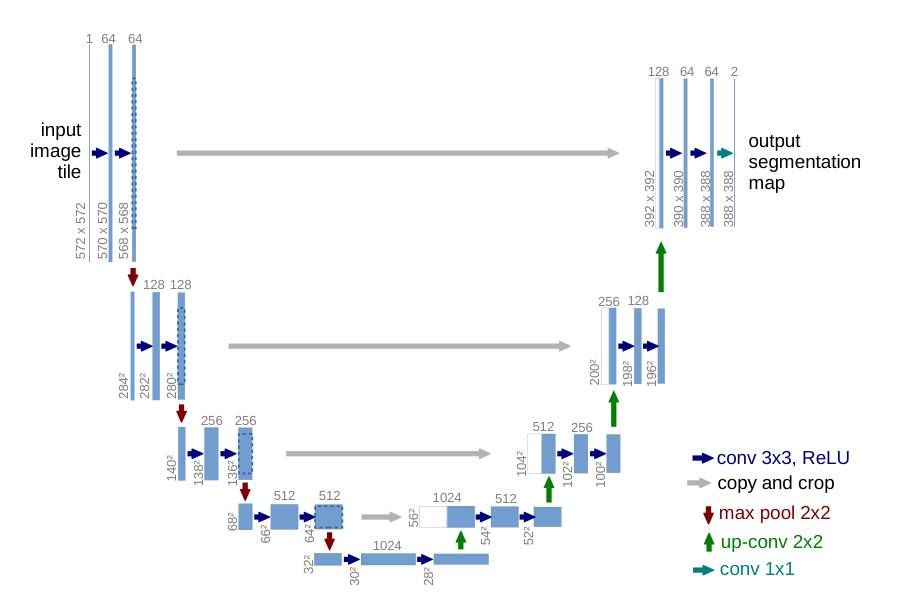
\includegraphics[width=0.7\textwidth]{Figures/chapter2/grasping/unet_encoder.png}
    \caption{U-Net encoder–decoder architecture (adapted from Ronneberger et al., 2015).}
    \label{fig:unet_arch}
\end{figure}

\textbf{U-Net} is a widely adopted encoder–decoder architecture that adds \textbf{skip connections} between matching encoder and decoder stages \cite{32}. These skip connections pass fine spatial detail directly to the decoder, improving localization while preserving global context \cite{32}. Although U-Net was originally introduced for biomedical segmentation, its design is broadly applicable to robotics perception tasks that require pixel-accurate outputs, such as \textbf{grasp quality maps} \cite{32}. In this project, the same encoder–decoder principle is used to predict grasp maps from RGB-D crops, where accurate localization of the grasp center is essential \cite{31, 32}.

\subsection{Residual Networks (ResNet) as Feature Extractors}
Deep residual networks (\textbf{ResNet}) introduce \textbf{identity skip connections} inside residual blocks, allowing the network to learn residual functions \cite{145}. This design improves gradient flow and enables the training of deeper backbones with better optimization stability \cite{145}.

\begin{figure}[H]
    \centering
    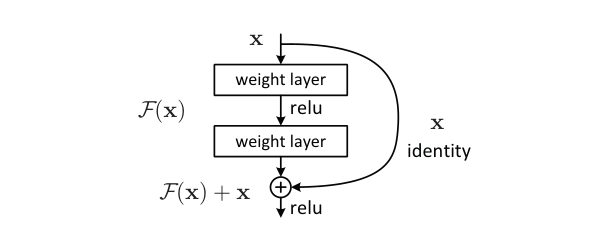
\includegraphics[width=0.5\textwidth]{Figures/chapter2/grasping/resnet.png}
    \caption{Residual learning building block and identity shortcut concept (from He et al., 2016).}
    \label{fig:resnet_block}
\end{figure}

In many vision pipelines, a ResNet is used as the encoder/backbone because it provides strong multi-scale features \cite{145}. When combined with a U-Net-style decoder, this produces a robust dense prediction network that can capture both global structure and local edges—useful for grasp inference on small objects such as bricks \cite{145}.

\subsection{Attention and Transformer Foundations}
\textbf{Transformers} replace recurrence and convolution with \textbf{attention mechanisms} that dynamically route information between tokens \cite{144}. In vision, tokens can represent image patches (ViT) or windowed patches (Swin) \cite{10}. The key operation is \textbf{self-attention}, where every token computes a weighted combination of other tokens based on content similarity \cite{9}.

\begin{figure}[H]
    \centering
    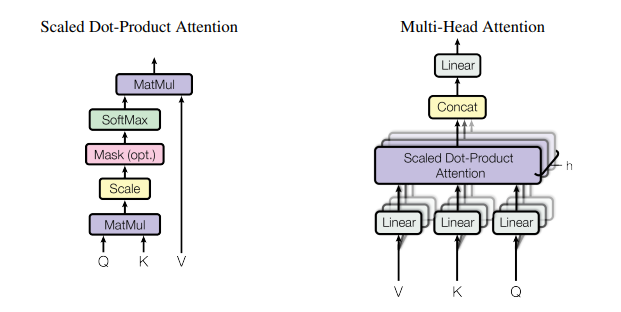
\includegraphics[width=0.7\textwidth]{Figures/chapter2/grasping/attention.png}
    \caption{(left) Scaled Dot-Product Attention. (right) Multi-Head Attention.}
    \label{fig:attention_mech}
\end{figure}

\subsection{Scaled Dot-Product Self-Attention}
Given an input sequence of token embeddings $X \in \mathbb{R}^{N \times D}$, self-attention first forms three projections: \textbf{queries (Q)}, \textbf{keys (K)}, and \textbf{values (V)} \cite{9}. The attention output is computed as:
\begin{equation}
    \text{Attention}(Q, K, V) = \text{softmax} \left( \frac{QK^T}{\sqrt{d_k}} \right) V
\end{equation}
Here, $d_k$ is the key dimensionality used for scaling \cite{9}. The matrix $A = \text{softmax}(QK^T / \sqrt{d_k})$ contains attention weights \cite{9}. Intuitively, keys describe what information a token offers, queries describe what information a token seeks, and values carry the content that will be aggregated \cite{9}.

\subsection{Multi-Head Attention (MHA)}
Instead of a single attention operation, multi-head attention splits the embedding into $h$ heads, runs attention independently in each head, and concatenates the results \cite{9}:
\begin{equation}
    \text{head}_i = \text{Attention}(QW_Q^i, KW_K^i, VW_V^i)
\end{equation}
\begin{equation}
    \text{MHA}(X) = \text{Concat}(\text{head}_1, \dots, \text{head}_h)W_O
\end{equation}
Multiple heads allow the model to attend to different patterns, such as edges, corners, and long-range relations, simultaneously \cite{9}.

\subsection{Vision Transformer (ViT)}
The \textbf{Vision Transformer (ViT)} adapts the Transformer encoder to images by representing an image as a sequence of patch tokens \cite{10}. 

\begin{figure}[H]
    \centering
    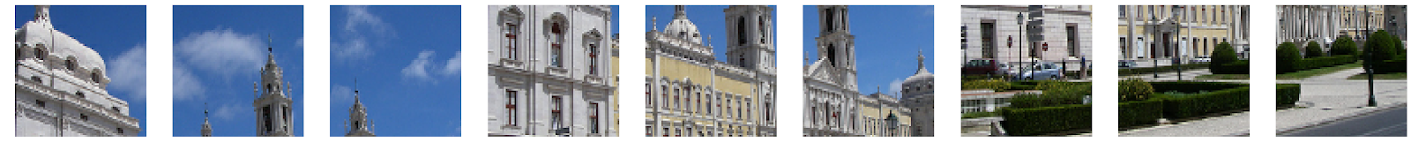
\includegraphics[width=0.8\textwidth]{Figures/chapter2/grasping/vit_overview.png}
    \caption{Vision Transformer (ViT) overview and patch-based tokenization (from Dosovitskiy et al., 2021).}
    \label{fig:vit_overview}
\end{figure}

An input image $I \in \mathbb{R}^{H \times W \times C}$ is split into non-overlapping patches of size $P \times P$ \cite{10}. Each patch is flattened and mapped to an embedding dimension $D$ using a learned linear projection \cite{10}. Because attention is permutation-invariant, ViT adds \textbf{positional embeddings} to encode patch locations \cite{10}. This allows the model to distinguish tokens by spatial position \cite{10}.

\subsection{Hierarchical Transformers: Swin}
A key challenge for vision is the quadratic cost of global attention with respect to the number of tokens \cite{3}. \textbf{Swin Transformer} addresses this by restricting attention to \textbf{local windows} and introducing \textbf{shifted-window attention} to enable cross-window interaction \cite{3}. The result is a hierarchical, multi-resolution feature pyramid that resembles CNN behavior while retaining attention-based modeling capacity \cite{3}.

\begin{figure}[H]
    \centering
    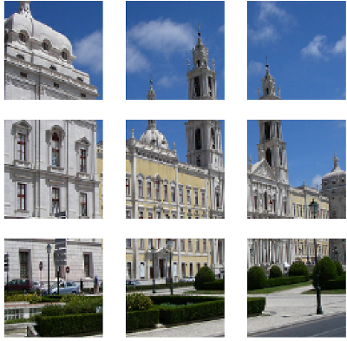
\includegraphics[width=0.7\textwidth]{Figures/chapter2/grasping/ViT.png}
    \caption{Swin Transformer hierarchical architecture and shifted-window self-attention concept (from Liu et al., 2021).}
    \label{fig:ViT}
\end{figure}

\subsection{Vision Transformer (ViT)}

\subsection{Patch Extraction and Patch Embedding}
The \textbf{Vision Transformer (ViT)} adapts the Transformer architecture to 2D images by treating them as sequences of tokens. An input image $I \in \mathbb{R}^{H \times W \times C}$ is split into non-overlapping patches of size $P \times P$ \cite{10}. The total number of patches, $N$, is calculated as:
\begin{equation}
    N = \frac{H \cdot W}{P^2}
\end{equation}

Each patch is flattened into a vector $x_p \in \mathbb{R}^{P^2 \cdot C}$ and mapped to an embedding dimension $D$ via a learned linear projection $E \in \mathbb{R}^{(P^2 \cdot C) \times D}$:
\begin{equation}
    z_p = x_p E
\end{equation}

For a $160 \times 160$ crop, using a patch size $P=16$ results in $N=100$ tokens, while $P=8$ provides $N=400$ tokens. While a smaller $P$ increases computational cost, it preserves significantly more \textbf{spatial detail}, which is critical for localizing small objects like bricks \cite{10}.



\subsection{Positional Encoding}
Because the attention mechanism is inherently permutation-invariant, ViT must explicitly encode spatial information. A learnable position vector $p_i$ is added to each patch token $Z_i$ to allow the model to distinguish tokens by their relative or absolute spatial position:
\begin{equation}
    \tilde{Z}_i = Z_i + p_i
\end{equation}

\subsection{Class Token vs. Dense Outputs}
While classification tasks typically prepend a \textbf{[CLS] token} to the sequence, dense prediction tasks (such as generating \textbf{grasp quality maps}) preserve all per-token features. These features are then processed by a lightweight decoder or a pyramid fusion module to reconstruct the pixel-wise grid.

\subsubsection{Computational Considerations}
Global self-attention possesses a computational complexity of $O(N^2)$, which grows quadratically with the number of tokens. This becomes computationally prohibitive for high-resolution images, motivating the development of window-based architectures like the Swin Transformer \cite{10}.

---

\subsubsection{Hierarchical Transformers: Swin}
The \textbf{Swin Transformer} addresses the quadratic scaling issue by restricting self-attention to \textbf{local windows}.

\begin{figure}[H]
    \centering
    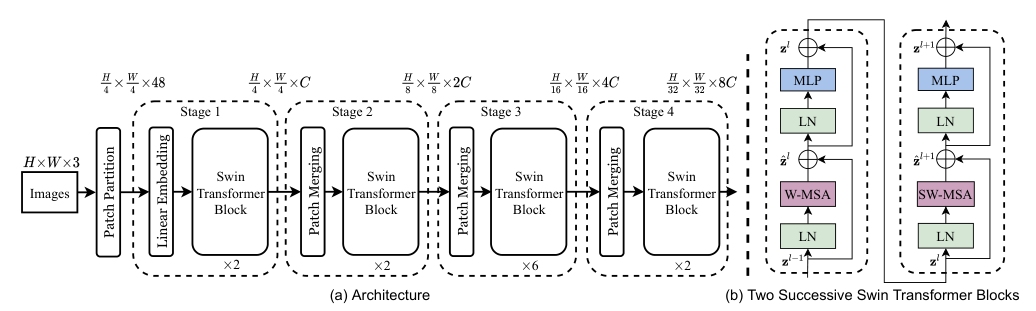
\includegraphics[width=0.8\textwidth]{Figures/chapter2/grasping/swin.png}
    \caption{Swin Transformer hierarchical architecture and shifted-window self-attention concept (from Liu et al., 2021).}
    \label{fig:swin_concept}
\end{figure}



\begin{itemize}
    \item \textbf{Shifted-Window Attention}: Introduces connections between neighboring non-overlapping windows by shifting the window partitions between consecutive layers \cite{3}.
    \item \textbf{Hierarchical Representation}: Unlike the fixed resolution of ViT, Swin produces a multi-resolution feature pyramid, similar to CNN backbones, making it a natural fit for dense prediction and multi-scale feature fusion \cite{3}.
\end{itemize}

---

\subsubsection{Summary of Prior Approaches in Robotic Grasp Prediction}
Robotic grasp prediction is generally categorized into discrete rectangle detection and \textbf{dense map prediction}.
\begin{itemize}
    \item \textbf{Dense Map Advantages}: Predicting grasp quality and orientation at every pixel allows for high-speed, real-time control via a simple \textbf{argmax} operation over the quality map.
    \item \textbf{Supervision}: Standard datasets such as the \textbf{Cornell Grasping Dataset} \cite{11} and \textbf{Jacquard} \cite{12} provide the ground-truth rectangles necessary to supervise these models.
    \item \textbf{Robustness}: Recent research emphasizes the integration of depth information and segmentation masks to improve performance under partial occlusions and workspace clutter.
\end{itemize}
